\subsection{K-Means}
\textit{written by B.L.}\\

\label{subsec:method_kmeans}
On the surface, the idea for K-Means clustering is straight forward: an initial grouping of observations closest to starting points, whereafter the starting points are updated to be placed at the center of these groupings. A new grouping step is performed and centers updated until the groupings do not change any further \cite{wiedenbeck2001klassifikation, fahrmeir2015multivariate}. This very brief introduction requires elaboration.\\

One way to look at clustering mathematically is to consider an objective function, similar to \cite{wu2012advances}
\begin{equation}
    \sum_{k=1}^{K}\sum_{x \in C_{k}}^{} w_{x}d(x, c_{k})
\end{equation}

where $K \in \mathbb{N}$ is the number of clusters $C_{k}, k \in \{ 1,\dots,K \}$ of which the centers are $c_{k}$. Observations are $x \in \mathcal{X}$ and their weights $w_{x}$ with $\mathcal{X} = \{ x_{1}, \dots, x_{m} \}$ being the entire data set. The data in $\mathcal{X}$ lives inside a feature space $\mathcal{F}^{n}$ with $n \in \mathbb{N}$ the number of different features. There also exists a measure on $\mathcal{F}^{n}$ that allows to calculate the distance $d$ between points. 

The most common specification of K-Means and often most practical in real world applications is the feature space being a euclidean space $\mathbb{R}^{n}$ and used for its distance function $d: \mathbb{R}^{n} \times \mathbb{R}^{n} \rightarrow \mathbb{R}$, fittingly, the euclidean distance (written as $\left \| \cdot \right \|$). Using these, the optimization problem presents as
\begin{equation}
\begin{gathered}
    \min \sum_{k=1}^{K}\sum_{x \in C_{k}}^{} \left \| x - c_{k} \right \|^2
\end{gathered}\label{eqn:kmeans_basic}
\end{equation}
\begin{equation}
\begin{gathered}
    = \min \sum_{k=1}^{K}\sum_{x \in C_{k}}^{} \left \| x - \frac{1}{\left | C_{k} \right |} \sum_{y \in C_{k}}^{} y  \right \|^2
\end{gathered}\label{eq:kmeans_basic_other}
\end{equation}

The inner sum in equation \ref{eqn:kmeans_basic} can be seen as the sum of squared errors (SSE) for each cluster. Notably this version omits the weighting of the points. Introducing (equal) weights for all points $(\dots)\sum_{x \in C_{k}}^{} \frac{1}{\left | C_{k} \right |} \left \| x - c_{k} \right \|^2$ will not change the clustering result but allows for it to be seen as the intra-cluster variance, its minimizaiton across clusters directly reflecting one of the objectives mentioned in section \ref{sec:problem_description}.

Achieving the goal described above globally is an NP-hard problem but convergence to local optima can be achieved rather efficiently. This leads to the question of how an approximation can be achieved in practice. A method similar to the one described by \cite{lloyd1982least,wu2012advances} works as follows:

The one parameter that has to be specified for this algorithm is $K$, the number of clusters one wishes to produce. Once a $K$ is chosen, the method can start by picking $K$ locations in the feature space $\mathcal{F}^{n}$ (each feature is a column in the data set). There are more advanced methods to be explored later but for the moment we assume these locations, so called centroids, $c_{k}$ to be picked randomly.
%For every observation $x$ in $\mathcal{F}^{n}$, there exists a distance $d_{n, c_{k}}$, calculated by a distance function $D$, to each of the centroids.
For every observation (row in the data) there is a centroid with the lowest distance (for equidistant centroids there is a method in place for assignment). In this step each observation is assumed to be part of the cluster $C_{k}$ whose centroid $c_{k}$ is closest to it. After this assignment the centroids are relocated to the "center" of their respective first step clusters (more on this below). Hereafter the method starts again from the point of calculating the distance between all observations and centroids. Observations are newly assigned to clusters, centroids are relocated and the method starts again. This procedure is repeated until the centroids are stationary (again, a closer look into this follows below). At this point a clustering has been achieved which satisfies the described method, but cannot necessarily be assumed to be the best clustering possible given the inputs. The entire procedure shall be redone from the top, beginning with new starting points, until one is reasonably satisfied with the stability of the result given a predefined method of evaluation. This series of operations can be summarized in a short amount of pseudo-code
\begin{algorithm}
\caption{Pseudo K-Means}\label{euclid}
\begin{algorithmic}[1]
\State place initial centroids $c_{i}$ \circled{1}
\While {centroids \textbf{not} stationary \circled{4}}
\If {observations have labels}
\State update centroids $c_{i}$ to center of current clusters $C_{i}$ \circled{3}
\EndIf
\State calculate all distances $d_{m, c_{i}}$ \circled{2}
\State assign each observation to min distant centroid via label $i$
\EndWhile
\end{algorithmic}
\end{algorithm}

where each of the numbers \circled{1} to \circled{4} refer to a topic mentioned above and further examined below.

Clustering with the described method is fast, commonly requiring fewer iterations than observations \cite{har2005fast}. The naive upper bound is trivially $\mathcal{O}(K^{n})$ (trying every possible configuration), with \cite{arthur2006slow} showing worst case run time to be superpolynomial ($\mathcal{O}(m^{(K+2/n)})$) with common runtimes being polynomial.

\circled{1} Initial placement of the centroids can be achieved in different ways. The most basic method is placing them at random. On singular runs of the algorithm this can lead to problems as can be seen in the example in Figure \ref{img:k_means_bad_init}. From a visual standpoint there should be three clusters, one to the left containing four observations, one in the middle containing two observations and one to the right with five observations. Initial random placement has resulted in two initial centroids far to the left and one near the center of the feature space. Performing the steps as described results in a final clustering of one cluster containing a single observation to the left, another comprising three observations also near the left and one big cluster with seven observations from two visually separated segments of the data. This is a valid result meeting stopping criteria but it is not meeting the expectations. Different starting positions can lead to different clustering results.

\begin{figure}[h]
\centering
%\includegraphics[width=0.6\textwidth]{something}
\resizebox{0.9\textwidth}{!}{
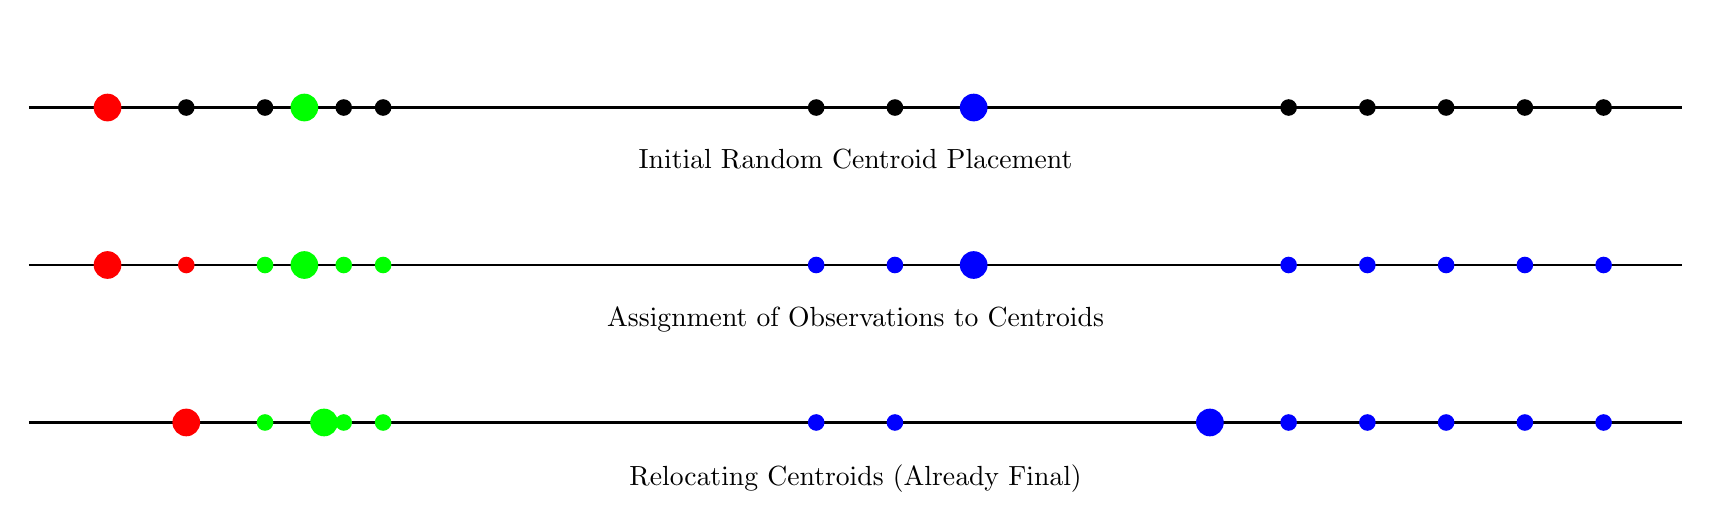
\begin{tikzpicture}[
dot/.style = {circle, fill=black,inner sep=0pt, minimum 
size=6pt},
bigdot/.style = {circle, fill=black, opacity=1, inner sep=0pt, minimum size=10pt},
every label/.append style = {inner sep=0pt, rotate around={45:(-0.5,1.5)}},
    thick      
                        ]
%spacing top
\draw[thick, opacity=0] (0,1) -- + (21,0);
%

% first line
\draw[thick] (0,0) -- node[below=4mm] {Initial Random Centroid Placement} + (21,0);
%
\foreach \p in {2, 3, 4, 4.5, 10, 11, 16, 17, 18, 19, 20}
{
    \node[dot] at (\p,0) {};
}

% first line centroids
\draw ( 1,0.0) -- + (0,-0.0) node[bigdot, fill=red] {};
\draw ( 3.5,0.0) -- + (0,-0.0) node[bigdot, fill=green] {};
\draw (12,0.0) -- + (0,-0.0) node[bigdot, fill=blue] {};

% second line
\draw[thick] (0,-2) -- node[below=4mm] {Assignment of Observations to Centroids} + (21,0);

%second line centroids
\draw ( 1,-2) -- + (0,-0.0) node[bigdot, fill=red] {};
\draw ( 3.5,-2) -- + (0,-0.0) node[bigdot, fill=green] {};
\draw (12,-2) -- + (0,-0.0) node[bigdot, fill=blue] {};

\draw ( 2,-2) -- + (0,-0.0) node[dot, fill=red] {};

\draw ( 3,-2) -- + (0,-0.0) node[dot, fill=green] {};
\draw ( 4,-2) -- + (0,-0.0) node[dot, fill=green] {};
\draw (4.5,-2) -- + (0,-0.0) node[dot, fill=green] {};

\draw (10,-2) -- + (0,-0.0) node[dot, fill=blue] {};
\draw (11,-2) -- + (0,-0.0) node[dot, fill=blue] {};

\draw (16,-2) -- + (0,-0.0) node[dot, fill=blue] {};
\draw (17,-2) -- + (0,-0.0) node[dot, fill=blue] {};
\draw (18,-2) -- + (0,-0.0) node[dot, fill=blue] {};
\draw (19,-2) -- + (0,-0.0) node[dot, fill=blue] {};
\draw (20,-2) -- + (0,-0.0) node[dot, fill=blue] {};

% third line
\draw[thick] (0,-4) -- node[below=4mm] {Relocating Centroids (Already Final)} + (21,0);

% third line centroids
\draw ( 2,-4) -- + (0,-0.0) node[bigdot, fill=red] {};
\draw ( 3.75,-4) -- + (0,-0.0) node[bigdot, fill=green] {};
\draw (15,-4) -- + (0,-0.0) node[bigdot, fill=blue] {};

\draw ( 3,-4) -- + (0,-0.0) node[dot, fill=green] {};
\draw ( 4,-4) -- + (0,-0.0) node[dot, fill=green] {};
\draw (4.5,-4) -- + (0,-0.0) node[dot, fill=green] {}; 

\draw (10,-4) -- + (0,-0.0) node[dot, fill=blue] {};
\draw (11,-4) -- + (0,-0.0) node[dot, fill=blue] {};

\draw (16,-4) -- + (0,-0.0) node[dot, fill=blue] {};
\draw (17,-4) -- + (0,-0.0) node[dot, fill=blue] {};
\draw (18,-4) -- + (0,-0.0) node[dot, fill=blue] {};
\draw (19,-4) -- + (0,-0.0) node[dot, fill=blue] {};
\draw (20,-4) -- + (0,-0.0) node[dot, fill=blue] {};

\end{tikzpicture}
}
\caption{One Dimension With Ten Observations - Bad Starting Positions}
\label{img:k_means_bad_init}
\end{figure}
%It can be seen that this initial placement does allow for \textit{a} clustering in the end, though it does not achieve what a human would describe as a fitting result. 
In two ways a solution to this problem can lie in repeating the method multiple times with different initialization. Firstly a new placement of initial centroids can lead to different clustering results which can be more fitting to the observer and secondly introducing a measure of fit and comparing it across runs to select the clustering that maximizes (minimizes) the measure can objectivize the selection of the "best" clustering. Commonly used as a measure are SSE and intra-cluster variance themselves, while other methods will be discussed more thoroughly in section \ref{sec:evaluation_description}. The repetition of clustering can therefore alleviate some problems introduced by randomly selecting starting points.

While computational capabilities are ever growing and trying more initializations should provide a higher chance of achieving better clustering results, it may still be useful to attempt improving on pure randomness.

One early proposition is selecting the center of the entire data set $\frac{1}{\left | \mathcal{X} \right |} \sum_{x \in \mathcal{X}}^{} x $ as a first centroid and then randomly going through all observations and picking the subsequent points if they exceed a predefined distance threshold \cite{ball1967clustering}.

To ensure that initial points cannot fall far from the data \cite{forgy1965cluster,jancey1966multidimensional} propose going a step further by only selecting observations as initial points by randomly selecting observations. This can save some iterations required to "pull" centroids towards the data and can prevent the formation of empty clusters. Assuming no inner logic to the ordering of data in a data set (which might of course exist and presents a problem to this method) an implementation of K-Means in SPSS \cite{noruvsis2011ibm} selects the first $i$ observations in the data set as starting points \cite{macqueen1967some}. 

A number of methods expand on the idea of working with observations by first selecting a single observation and then seeking to select more not too close to the first one, which appears sensible computationally as well as considering the goal of identifying seperate clusters.

One such idea is to randomly select a starting point and subsequently selecting points with the maximum minimal distance to the previously selected \cite{gonzalez1985clustering}, often called \textit{maximin}.

A popular method going by the name \textit{kmeans++} developed by \cite{arthur2006k} extends the idea by \cite{macqueen1967some} described above. After arbitrarily selecting a first observation, the remaining $K-1$ initial points are picked in a random process. Instead of assuming an even distribution all observations are assigned probabilities proportional to the squared distance to their nearest previously picked initial centroid. Despite the additional computational aufwand in the beginning, this method shows reductions in terminal errors as well as time to convergence of up to half compared to naive random selection on $\mathcal{F}^{n}$. There are implementations of \textit{kmeans++} for most popular machine learning implementations, including the one described in section \ref{sec:python_description}.
This selection of methods is by no means exhaustive but should give a good overview of popular options.

\circled{2} In theory the practical application of the algorithm described above can be adapted to a plethora of distance measures to varying degrees of success. As described the most natural is the euclidean distance as it maps directly to variance minimization. It has been shown by \cite{aggarwal2001surprising} that other $L^{p}$ norms than $L^{2}$ (like euclidean) can be used successfully, $L^{1}$ proving particularly good when applied for high dimensional cases. It can be shown by \cite{selim1984k}, though, that using metrics other than euclidean distances may cause the method to fail to converge. This may in some cases be alleviated by a clever selection of thresholds as described in \circled{4}.
The choice of distance function will affect the clustering result. Opting for the euclidean distance will lead to clusters tending towards \textit{n-spherical} shapes, applying Manhattan distance \textit{hyper cubes} and so on. Befitting the K-Means designation the ideal use case is data containing mostly contiguous subsets distributed around a finite number of means. Illustration \ref{img:k_means_cluster_success} depicts examples of data suitable (1,3) and not suitable (2,4,5) for K-Means application \cite{sklearn_website}.

\begin{figure}[h]
\centering
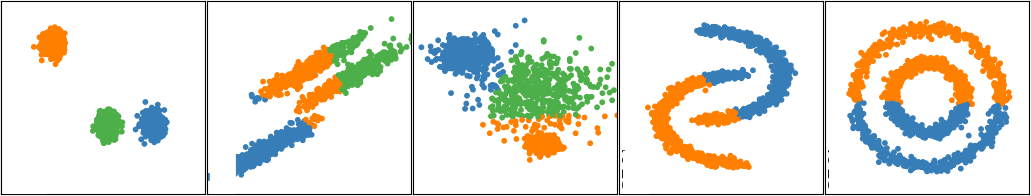
\includegraphics[width=0.75\textwidth]{images/kmeans_suitable_shapes.png}
\caption{Data Shapes and K-Means Clustering Success}
\label{img:k_means_cluster_success}
\end{figure}

\circled{3} The K-Means name makes it sufficiently clear that the selected method of calculating the position of centroids is by taking the mean of the observations grouped in the particular cluster. However, other interpretations of the concept of a mean have been devised in order to tackle specific limitations of the described method. One of the best known is \textit{K-Medoids}. A method described similar to K-Means by \cite{park2009simple} proposes to always select the most central observations of each cluster by minimizing the sum of pairwise dissimilarities. This method is generally more robust to outliers and can perform better when incorporating categorical data.

\circled{4} An important question to answer is when to stop iterating. There are mainly three options (cf. \cite{cleuziou2008extended}): Execution can be stopped once the centroids stop changing. It is possible though to construct examples where this is unlikely to happen. Then this criterion can be expanded to stopping when the distance of centroids between iterations is below a threshold like \cite{lloyd1982least} suggests. Another idea is to stop execution when intra-cluster variance (or another measure) stops improving, respectively improves less than a threshold, for a defined number of iterations. The third option is to stop when points remain in the same cluster for multiple iterations. In many software implementations there is an option to hard cap the number of iterations to prevent excessively long execution times or simply in place of one of the described criteria.\\

The elephant in the room remains: how to choose $K$? Looking at equation \ref{eqn:kmeans_basic} makes it obvious that optimization improves when increasing $K$. It is also obvious that simply adding more clusters is not the goal. Domain knowledge about the data set can inform the decision but the application case for an unsupervised method like K-Means typically lacks this type of information. A brief overview of methods to determine $K$ by \cite{pham2005selection, yuan2019research} include among others: visualizing the clustered data, density, internal validation measures (see section \ref{sec:evaluation_description}), gap statistic, or their own distortion measure. One common method of determining $K$ from these statistical methods is then to apply the so-called \textit{elbow rule}: clustering is performed for multiple different $K$ and the corresponding statistics are calculated. The results are then plotted against each other. Often the resulting plot exhibits a "kink" at a certain point after which its trajectory flattens out. Its position then is used as an approximation of $K$. Viability of this method varies depending on the underlying data.